
\section{Suma niespójna i~suma spójna}

\begin{definition}[suma niespójna]
% DICTIONARY;distant union;suma niespójna;-
\index{suma niespójna}%
    Niech $L_1$ oraz $L_2$ będą splotami, które leżą po różnych stronach ustalonej płaszczyzny w przestrzeni $\R^3$.
    Teoriomnogościową sumę $L_1 \sqcup L_2$ nazywamy sumą niespójną splotów $L_1$ i $L_2$.
\end{definition}

\begin{definition}[suma spójna]
% DICTIONARY;connected sum;suma spójna;-
\index{suma spójna}%
\label{def:connected_sum}%
    Niech $K_1, K_2$ będą zorientowanymi węzłami.
    Natnijmy każdy z nich w dwóch punktach tego samego krótkiego łuku, a następnie zszyjmy dwoma łukami, które nie przecinają już istniejących, jak na obrazku.
    Otrzymany węzeł nazywamy sumą spójną węzłów $K_1$ oraz $K_2$ i oznaczamy przez $K_1 \shrap K_2$.
\end{definition}

\begin{example}
    Suma spójna $10_{17} \shrap 9_{44}$:
    \[
        \raisebox{-0.42\height}{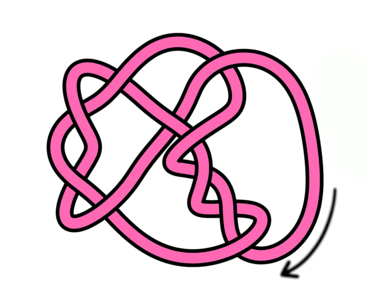
\includegraphics[height=2.2cm]{../data/connected-sum/knot_sum_a.png}}
        \scalebox{2.5}{\ensuremath{\shrap}}
        \raisebox{-0.42\height}{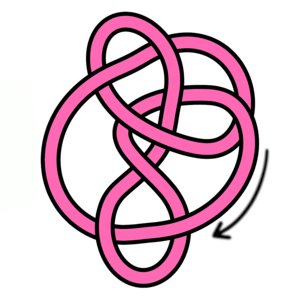
\includegraphics[height=2.2cm]{../data/connected-sum/knot_sum_b.png}}
        \scalebox{2.5}{\ensuremath{=}}
        \raisebox{-0.42\height}{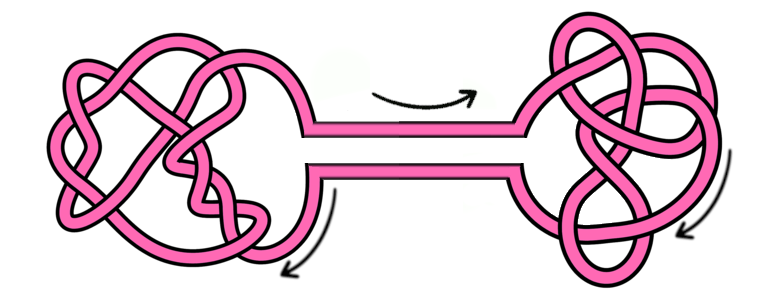
\includegraphics[height=2.2cm]{../data/connected-sum/knot_sum_ab.png}}
    \]
\end{example}

W topologii rozważa się podobną operację: z~każdej $n$-rozmaitości wycina się kulę, po czym skleja wzdłuż brzegowej sfery w~jedną rozmaitość.
Ale kiedy zajmujemy się węzłami, nie interesuje nas struktura rozmaitości (gdyż każdy węzeł jest homeomorficzny z~okręgiem), tylko zanurzenie w otaczającą przestrzeń.
Pojęcie sumy spójnej węzłów (oraz opisane później satelity) wprowadził do matematyki Schubert \cite{schubert1949}.
\index[persons]{Schubert, Horst}%

Żadnego elementu definicji \ref{def:connected_sum} nie można pominąć:
\begin{itemize}
    \item \emph{składniki $K_1, K_2$ muszą być zorientowane}. 
    Węzeł prosty, czyli suma dwóch przeciwnie skręconych trójlistników, ma zerową sygnaturę i jest plastrowy.
    \index{węzeł!plastrowy}%
    \index{sygnatura}%
    Węzeł babski, czyli suma tak samo skręconych trójlistników ma niezerową sygnaturę.
    (To jedno z niewielu miejsc, gdzie nomenklatura pochodzi od żeglarzy.).
    \label{two_sums_of_two_trefoils}%
    Uzasadnienie, że te węzły są różne, nie jest łatwym zadaniem.
    Fox twierdzi, że Seifert \cite{seifert1933} wiedział o tym.
    Pokazał też w~króciutkim artykule \cite{fox1952}, że ich dopełnienia nie są homeomorficzne.
    \item \emph{składniki $K_1, K_2$ muszą być węzłami, nie splotami}. Nie istnieje kanoniczny wybór, które ogniwa łączyć ze sobą.
    \item \emph{zszywajace łuki nie mogą przecinać diagramów}.
    Cromwell \cite[s. 90]{cromwell2004} pokazuje przykład dwóch niewęzłów, z~których otrzymano niepoprawnie dwie różne sumy, $6_1$ oraz $8_{20}$.
\end{itemize}

\begin{proposition}
    Suma spójna węzłów jest dobrze określonym działaniem.
    Jest przemienna oraz łączna; niewęzeł stanowi jej element neutralny.
\end{proposition}

\begin{proof}
    Niech dane będą węzły $K_1$ oraz $K_2$ oraz dwa różne łuki $\gamma_1$, $\gamma_2$, których można użyć do konstrukcji sumy spójnej.
    Skurczmy $K_1$ tak, by był bardzo mały, przeciągnijmy najpierw przez łuk $\gamma_1$, a~następnie wzdłuż węzła $K_2$ do miejsca, gdzie zaczyna się łuk $\gamma_2$.
    Na koniec odwróćmy proces, z łukiem~$\gamma_2$ w~miejscu łuku $\gamma_1$.

    Prosty dowód drugiego zdania pozostawiamy Czytelnikowi.
\end{proof}

Algebra powiedziałaby, że węzły z~sumą spójną tworzą półgrupę, podobnie jak liczby naturalne z~działaniem dodawania.
Do bycia grupą brakuje istnienia elementów przeciwnych. 
Znane są nam co najmniej trzy różne sposoby na uzasadnienie tego faktu.

Najpierw wywnioskowaliśmy to z~własności powierzchni Seiferta i~ich genusu: faktów \ref{prp:genus_detects_unknot} oraz \ref{prp:genus_of_sum}.
O~tym samym dowodzie wspomina Kawauchi \cite[s. 33]{kawauchi1996}, a~fakt nazywa twierdzeniem o~nieanulowaniu.
Potem poznaliśmy szwindel Mazura, technikę dowodzenia bardziej przystępną dla kogoś, kto nie zna topologii algebraicznej, ale niestety wykorzystującą węzły dziki.
Długo myśleliśmy, że inaczej się nie da, ale elementarny dowód istnieje!
% odkryte w https://aperiodical.com/2018/07/the-big-internet-math-off-round-1-jim-propp-v-zoe-griffiths/
Trzeba zajrzeć do \cite[s. 18-20]{kauffman1995} dla dwóch rysunków tamże.

\begin{proposition}
\label{first_time_sum_is_trivial}%
    Niech $K_1, K_2$ będą takimi węzłami, że $K_1 \shrap K_2 = \SmallUnknot$. Wtedy $K_1 = K_2 = \SmallUnknot$.
\end{proposition}

\begin{proof}[Niedowód]
% DICTIONARY;Mazur swindle;szwindel Mazura;-
    Technika ta zwana jest szwindlem Mazura.
\index{szwindel Mazura}%
    Załóżmy, że $K \shrap L = \SmallUnknot$ i~dopuśćmy wyjątkowo węzły dzikie.
    Skonstruujmy sumę $K \shrap L \shrap K \shrap \ldots$,
    przy czym kolejne składniki powinny zmniejszać się,
    aby ich suma nadal była węzłem.
    Wtedy
    \begin{align*}
        K & \simeq K \shrap [(L \shrap K) \shrap (L \shrap K) \ldots] \\
         & \simeq (K \shrap L) \shrap (K \shrap L) \shrap \ldots
         \simeq \SmallUnknot \shrap \SmallUnknot \shrap \ldots
         \simeq \SmallUnknot.
    \end{align*}
    Analogicznie pokazujemy, że $L \simeq \SmallUnknot$.
    To jedyne miejsce w~całej książce, gdzie użyte zostają (zostały?) węzły dzikie.
\end{proof}

\begin{proof}
    (Jak pan Kauffman \cite[s. 18-20]{kauffman1995} napisał).
    Wyobraźmy sobie, że węzeł oraz torus połykająco-podążający $T$ został zawieszony między dwiema ścianami pokoju i~załóżmy nie wprost, że suma $K = K_1 \shrap K_2$ jest trywialna.
    Wtedy pewien homeomorfizm pokoju, który nie rusza ścian, prostuje sumę: zamienia pozornie zaplątany węzeł $K$ w odcinek $L$. 

    Niech $\pi$ będzie dowolną płaszczyzną zawierającą wyprostowaną sumę $K$.
    Tnie część wspólną torusa $T$ oraz ścian w czterech punktach, oznaczmy je $A, B$ (na lewej ścianie) oraz $C, D$ (na prawej).
    Zauważmy, że $\pi$ tnie $T$ w łukach, które wychodzą z $A, B, C, D$ oraz pewnych zamkniętych krzywych.
    Łuk wychodzący z~punktu $A$ nie może łączyć go z punktami $B$ lub $D$, ponieważ te leżą po drugiej stronie odcinka $L$ na płaszczyźnie $\pi$.
    
    Łuk $AC$ przedstawia niewęzeł.
    Jednocześnie jest on obrazem pewnego łuku, który łączył końce torusa $T$, zatem musi być równoważny z~węzłem-towarzyszem.
\end{proof}

Półgrupę węzłów z~operacją sumy spójnej można uczynić grupą na dwa sposoby: albo zmieniając działanie, albo osłabiając równoważność węzłów.
Drugi pomysł jest lepszy niż pierwszy.
Na początku lat pięćdziesiątych Milnor wprowadził pojęcie zgodności.
\index[persons]{Milnor, John}%
\index{węzeł!plastrowy}%
\index{węzeł!zgodny}%
Element neutralny nowej grupy to węzły plastrowe, ich opis leży w~sekcji \ref{sec:slice}.
Zgodność i plastrowe węzły to zagadnienia zakorzenione w~czterowymiarowej topologii.

Kawauchi \cite[s. 50-53]{kawauchi1996} opisuje $2n$-sumę Murasugiego tak, że $2$-suma to nasza suma spójna, zaś $4$-suma to \textsc{,,plumbing''} (coś, czego nie znamy) i dodaje komentarz, że jest bardzo przydatna do badania powierzchni Seiferta czy genusu.
\index{plumbing}%
\index{suma Murasugiego}%
Została wprowadzona dawno temu w~\cite{murasugi1958}, by szacować stopień wielomianu Alexandera alternujących węzłów.
\index[persons]{Murasugi, Kunio}%
\index{wielomian Alexandera}%
\index{sploty alternujące}%

% DICTIONARY;suma paskowa;band sum;-
Innym uogólnieniem jest suma paskowa, patrz \cite[s. 31-32, 43]{kawauchi1996}, specjalny przypadek hiperbolicznej transformacji splotu oraz fuzji splotu.
\index{suma paskowa}%
% TODO: sprawdzić, czy fuzja splotu ma trafić do indeksu

% Koniec podsekcji Suma niespójna i suma spójna

